
\section{Injection, surjection and bijection}
You may have noticed in the previous exercise that question 2 is particularly \\ interesting. There is a restriction on the domain of \(h(x)\). Why is that? This is what this chapter is all about. However, before we explain that, I will go over some definitions of properties of functions. Firstly, we have \textit{injection}. 
\begin{definition}{Injective functions}{}
  An \textbf{injective} function, \(f\), or a \textit{one-to-one} function, is a function such that every distinct output of the function corresponds to only \textit{one} distinct input, that is \sidenotemark:  
  \begin{equation*}
    f(x_1) = f(x_2) \text{\, implies \,} x_1 = x_2 
  \end{equation*}
\end{definition}
\sidenotetext{\footnotesize \textit{By contraposition, \(x_1 \neq x_2\) implies \(f(x_1) \neq f(x_2)\). The contraposition of a statement "p then q" is "not q then p".}}
Of course, this explanation might not have been very clear. Here is a visualization:
\begin{figure}[h]
  \centering
  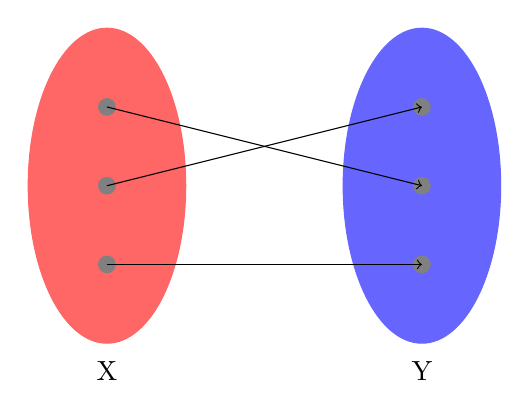
\begin{tikzpicture}
    \filldraw [red!60] (0,0) ellipse (1cm and 2cm) node[below, yshift=-60, color=black]{X}; 
    \filldraw [blue!60] (4,0) ellipse (1cm and 2cm) node[below, yshift=-60, color=black]{Y};
    \filldraw [gray] (0,1) circle (3pt);
    \filldraw [gray] (0,0) circle (3pt);
    \filldraw [gray] (0,-1) circle (3pt);
    \filldraw [gray] (4,1) circle (3pt);
    \filldraw [gray] (4,0) circle (3pt);
    \filldraw [gray] (4,-1) circle (3pt);
    \draw[->, black] (0,1) -- (4,0);
    \draw[->, black] (0,0) -- (4,1);
    \draw[->, black] (0,-1) -- (4,-1);
  \end{tikzpicture}

  \caption{Illustration of an injective function with domain \(X\) and range \(Y\).}
  \label{inj}
\end{figure}


As you can see in \Cref{inj}, every output in \(Y\) of the function is associated with only one input in \(X\), hence the function is \textit{injective}. (Kind of like how marriages \textit{should} be.) To prove that a function \(f\) is injective, you can either show that if \(x_1 \neq x_2\), then \(f(x_1) \neq f(x_2)\), or if \(f(x_1) = f(x_2)\), then \(x_1 = x_2\).

\begin{figure}[h]
  \centering
  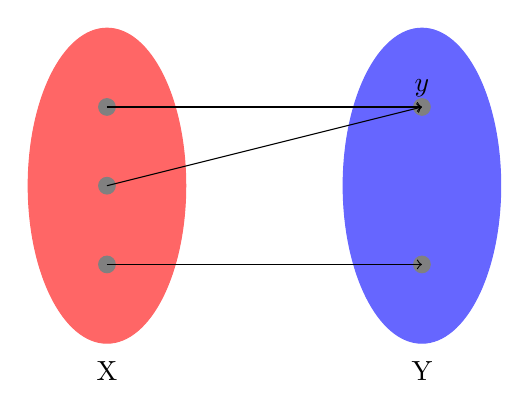
\begin{tikzpicture}
    \filldraw [red!60] (0,0) ellipse (1cm and 2cm) node[below, yshift=-60, color=black]{X}; 
    \filldraw [blue!60] (4,0) ellipse (1cm and 2cm) node[below, yshift=-60, color=black]{Y};
    \filldraw [gray] (0,1) circle (3pt);
    \filldraw [gray] (0,0) circle (3pt);
    \filldraw [gray] (0,-1) circle (3pt);
    \filldraw [gray] (4,1) circle (3pt) node[above, color=black]{\(y\)};
    \filldraw [gray] (4,-1) circle (3pt);
    \draw[->, black] (0,1) -- (4,1);
    \draw[->, black] (0,0) -- (4,1);
    \draw[->, black] (0,-1) -- (4,-1);
  \end{tikzpicture} 
  \caption{Illustration of a non-injective function with domain \(X\) and range \(Y\).}
  \label{non_inj}
\end{figure}


Here, the function is \textit{not} injective. As you can see in \Cref{non_inj}, the output \(y\) is associated with more than one input in \(X\). With this in mind, it is time to talk about \textit{surjection}. 
\begin{definition}{Surjective function}{}
  A \textbf{surjective} function \(f\) is a function such that for every output \(y\), there exists at least one input \(x\) such that \(f(x)=y\). 
\end{definition}


From \Cref{inj} and \Cref{non_inj}, both functions are surjective as every output is \\ associated with at least one input. Do take note that it does not matter how many inputs associate to one output, as long every output is associated with at least one input, the function is surjective. To prove that a function is surjective, you must show that there exists an element in the domain of the function for any arbitrary output in the range.

\begin{figure}[h]
  \centering
  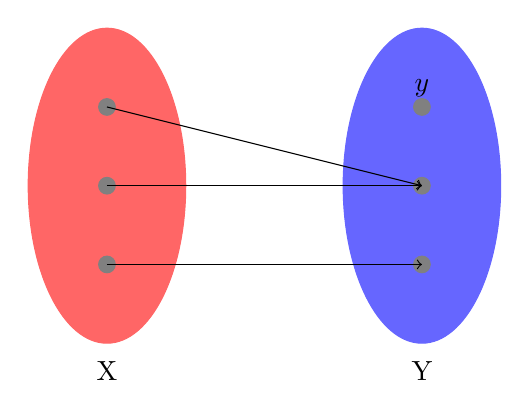
\begin{tikzpicture}
    \filldraw [red!60] (0,0) ellipse (1cm and 2cm) node[below, yshift=-60, color=black]{X}; 
    \filldraw [blue!60] (4,0) ellipse (1cm and 2cm) node[below, yshift=-60, color=black]{Y};
    \filldraw [gray] (0,1) circle (3pt);
    \filldraw [gray] (0,0) circle (3pt);
    \filldraw [gray] (0,-1) circle (3pt);
    \filldraw [gray] (4,1) circle (3pt) node[above, color=black]{\(y\)};
    \filldraw [gray] (4,0) circle (3pt);
    \filldraw [gray] (4,-1) circle (3pt);
    \draw[->, black] (0,1) -- (4,0);
    \draw[->, black] (0,0) -- (4,0);
    \draw[->, black] (0,-1) -- (4,-1);
  \end{tikzpicture} 
  \caption{Illustration of non-surjective function with domain \(X\) and range \(Y\).}
  \label{nsurj}
\end{figure}


From \Cref{nsurj}, we can see that \(y\) has no input associated with it. As a result, the function here is not surjective. Lastly, \textit{bijective} functions can't be any easier.
\begin{definition}{Bijective function}{}
  A \textbf{bijective} function is a function that is both injective and surjective. 
\end{definition}


However, bijective functions have a superpower. A function is only bijective \textit{if and only if} it has an inverse. \marginnote{\footnotesize \textit{P iff Q, or "P if and only if Q", means that "if P then Q" and "if Q then P".}}
\begin{theorem}{Bijection and inverses}{}
  A function, \(f:A \to B\), has an inverse if and only if it is bijective.
\end{theorem}
\begin{proof}{Bijection and inverses}{}
  To begin such proofs where there is a "if and only if" clause, we will prove both cases separately. First, we claim that if the function has an inverse, then it is bijective. To prove this, we simply prove that \(f\) is injective and surjective. Then, we claim that if a function is bijective, then it has an inverse. With both proofs below, we show that \(f\) has an inverse if and only if it is a bijection.
\end{proof}
\begin{lemma}{Inverse function has bijections}{}
  If a function, \(f: A \to B\), has an inverse, then it is bijective. 
  \label{inversebiject}
\end{lemma}
\begin{proof}{Inverse functions has bijections}{}
  Suppose \(f^{-1}\) is the inverse of \(f\). Notice that \(f^{-1}(f(x))\) is injective as it is simply \(f(x)=x\). Suppose \(a, a^\prime \in A\) and \(f(a)=f(a^\prime)\), then \(f^{-1}(f(a))=f^{-1}(f(a^\prime)))\). Notice that by injectivity of \(f^{-1}(f(x))\), \(a=a^\prime\). Hence, \(f\) is injective. Then, suppose \(b \in B\), we wish to show that the function is surjective. Also, \(f(f^{-1}(x))\) is surjective(it is the identity function). Let \(f^{-1}(b)=x\) and \(f(f^{-1}(b))=c\) for some \(c \in B\). By a simple substitution, \(f(f^{-1}(b))=f(x)=c\), thereby showing there exists a \(x \in A\) for every \(c \in B\). The two cases proves that \(f\) is bijective if it has an inverse.
\end{proof}
\begin{lemma}{Bijective function has inverses}{}
  If a function, \(f: A \to B\), is a bijection, then it has an inverse.
  \label{bijectinverse}
\end{lemma}
\begin{proof}{Bijective function has inverses}{}
  Let us define \(f^{-1}\) as \(f^{-1}: B \to A\). Let \(b \in B\). Since \(f\) is surjective, there exists \(a \in A\) such that \(f(a)=b\). Let \(f^{-1}(b)=a\). Since \(f\) is injective, \(f^{-1}\) is well-defined, or a function that outputs the same value given the same input. Next, we will show that \(f^{-1}\) is indeed the inverse of \(f\) by showing the composition of the two is an identity function. Again, let \(a \in A\) and \(b=f(a)\) which implies, by definition, \(f^{-1}(b)=a\). Composing the two functions, \(f(f^{-1}(b))=f(a)=b\), which shows that \(f^{-1}\) is indeed the inverse function. The other case of \(f^{-1} \circ f\) is similar. Hence, if \(f\) is a bijection, then it has an inverse.
\end{proof}
\begin{remark}{}{}
  This serves as a very good example showing how the reader should prove the injectivity, surjectivity, and bijectivity of functions. Also, this explains why in the previous exercise, the function \(h(x)=(x-7)^2\) is bounded, only taking \(x\) values larger than 7. The function is not bijective in \(\mathbb{R}\), as evident in the graph as it is not injective. Hence, the bounds are needed for \(h\) to have an inverse.
\end{remark}
\begin{marginfigure}
  \centering
  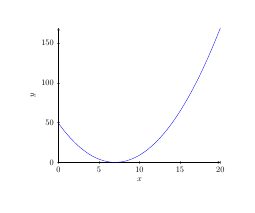
\begin{tikzpicture}[scale=0.3, samples=50]
    \begin{axis}[xlabel=\(x\), ylabel=\(y\), axis lines=left, domain=0:20]
      \addplot[mark=none, color=blue]{(x - 7)^2}; 
    \end{axis} 
  \end{tikzpicture}
  \caption{Plot of \((x-7)^2\).}
\end{marginfigure}
\hrule
\begin{problem}
  Determine if the following functions are injective or surjective or bijective in its domain:
  \begin{enumerate}[label=\alph*)]
    \item{\(f(x)=\sqrt{x}, f: \mathbb{R}^{+} \to \mathbb{R}^{+}\)}
    \item{\(f(x)=\frac{1}{x}, x>0\)}
    \item{\(f(x)=(x-7)^2, x \geq 5\)}
  \end{enumerate}
\end{problem}
\begin{problem}[1]

  Prove that:
  \begin{enumerate}[label=\alph*)]
    \item{The composition of two injective functions is \textit{injective}.}
    \item{The inverse of a function is \textit{injective}.}
    \item{The inverse of a function is \textit{surjective}.}
  \end{enumerate}
\end{problem}
\begin{problem}[1]
  Given a quadratic function \(q(x)=ax^2+bx+c\), and \(a\neq 0\), show that \(q\) cannot be bijective.
\end{problem}

\subsubsection*{Further problems}
\hrule
\begin{problem}[1]
  \textit{(Polynomial remainder theorem)} Let \(f(x)\) be a polynomial. If \(f(a)=0\), prove that \(x-a\) is a factor of \(f(x)\).
\end{problem}
\begin{problem}[1]
  We shall define an area function, \(A(f,x_1,x_2)\) which gives us the area under a given function \(f(x)\) \sidenote{\footnotesize\textit{If you are skeptical about the area function provides the area for any function, you are absolutely right. This property that a function can be integrated is called integrability. If you are interested, there are many types, such as the physicist favourite "square-integrability". However, the point of the problem remains.}} bound by \(x_1\leq x\leq x_2\).
  \begin{enumerate}[label=\alph*)]
    \item{Using an example, show that \(A(f,x_1,x_2)\) cannot be bijective.}
    \item{Also using an example, disprove that \(A(fg,x_1,x_2)=A(f,x_1,x_2)A(g,x_1,x_2)\).}
    \item{From the examples, verify geometrically that \(A(f+g,x_1,x_2)=A(f,x_1,x_2)+A(g,x_1,x_2)\):
      \begin{enumerate}
        \item{\(f(x)=x+1\) and \(g(x)=x+2\)}
        \item{\(f(x)=x\) and \(g(x)=0\)}
        \item{\(f(x)=1\) and \(g(x)=2\)}
      \end{enumerate}
      }
    \item{If \(\delta\) is the dirac delta function found in Problem \ref{diracpb}, show that \(A((x^2+x+1)\delta(x-1),-\infty, \infty)=3\). It is given that \(A(cf(x),\ldots)=cA(f(x),\ldots)\) for some constant \(c\).}
  \end{enumerate}
\end{problem}
\begin{problem}[2]
  The \textit{wavefunction} \(\Psi\) of a particle can be thought of as the quantum state of a particle. In this problem, you will solve for the wavefunction of an one-dimensional particle (that lies on the x-axis) in an infinite square well. It is given that \(|\psi(x)|^2\) gives the probability of the particle existing at \(x\) and \(|\Psi(x,t)|^2\) is the probability of a particle existing at \(x\) at time \(t\). (Hence, note that \(\Psi(x)\neq 0\) and \(\psi(x)\neq 0\). That would imply that the particle cannot be found anywhere.) The potential function of the infinite square well is
  \begin{equation}
    V(x) = \begin{cases}
      0 & 0\leq x\leq a \\
      \infty & \textit{otherwise}
    \end{cases}
  \end{equation}
  \begin{enumerate}[label=\alph*)]
    \item{Can the particle exist outside of \(0\leq x\leq a\), or more specifically, what is \(|\psi(x)|^2\) (and therefore \(\psi(x)\)) for \(x<0\) or \(x>a\)?}
    \item{To ensure that \(\psi\) is continuous, \(\psi(0)\) and \(\psi(a)\) are equal to your answer of \(\psi(x)\) in (a). Also, it is known that the form of general solution inside the well (to wit: \(0\leq x\leq a\)) to \(\psi\) is \(\psi(x)=A\sin(kx)+B\cos(kx)\). Show that \(\psi(x)=A\sin(kx)\).}
    \item{Using your answer in (b), solve for \(k\). (Hint: k has multiple solutions, generalize all the solutions by writing down \(k_n\) for \(n\in \mathbb{Z}\setminus\{0\}\).)}
    \item{Show that we can discard all negative solutions of \(k_n\), hence \(n\in \mathbb{N}\).}
    \item{If \(E(n)=\frac{\hbar^2 k_n^2}{2m}\), find \(E(1)\) or the energy of the \textit{ground state} of the particle. \(\hbar\) is the reduced plank's constant. What happens as \(n\) increases?}
    \item{The relation between \(\Psi\) and \(\psi\) is \(\Psi(x,t)=\psi(x)e^{-\frac{iE(n)t}{\hbar}}\). Find \(|\Psi|^2\) for \(t=1\) and \(t=2\), what happens to the graph of \(|\Psi|^2\) as time passes? Take \(A, m, a\) as positive real numbers and choose some natural \(n\).}
  \end{enumerate}
  \label{infinitewell}
\end{problem}
\begin{problem}[3]
  If \( f(x)=2^{x}-x \), find \(x_1\) such that \( f(x_1)=5\).
\end{problem}
% \begin{enumerate}
%   \item{
%       \begin{enumerate}
%         \item{Bijective}
%         \item{Injective}
%         \item{Surjective}
%       \end{enumerate}
%     } 
%   \item{
%       \begin{enumerate}
%         \item{Let the two functions be \(f: A \to B\) and \(g: B \to C\). If \(g(f(x_1))=g(f(x_2)))\), by injectivity of \(g\), \(f(x_1)=f(x_2)\) and by injectivity of \(f\), \(x_1=x_2\). Thus, \(g \circ f\) is injective.}
%         \item{Let \(f:A \to B\) and \(f^{-1}\) be its inverse. Notice if \(f^{-1}(x_1)=f^{-1}(x_2)\), then \(f(f^{-1}(x_1))=f(f^{-1}(x_2))\) which implies \(x_1=x_2\). Hence, \(f^{-1}\) is injective.}
%         \item{Similarly, define \(f\) and \(f^{-1}\). Let \(y \in A\) and \(f^{-1}(x)=y\). Notice that \(x=f(y)\) and because \(f\) is surjective(by \Cref{inversebiject}), \(x \in B\), thus proving that \(f^{-1}\) is surjective.}
%       \end{enumerate}
%     }
% \end{enumerate}  
